\chapter{BotScope: progettazione} \label{chap:progettazione} % 4

% Questo capitolo ha l'obiettivo di presentare l'architettura proposta per risolvere il problema affrontato in questi tesi. In primo luogo verrà mostrata l'architettura generale, utilizzando un diagramma dei componenti, e successivamente, per ciascun componente, verranno individuate le caratteristiche principali. Infine, verrà descritto il funzionamento del sistema da un ulteriore punto di vista, illustrando un flusso di esecuzione completo mediante un diagramma delle attività e approfondendo il meccanismo di \textit{tool calling} con un diagramma di sequenza.

\section{Architettura del sistema} % 4.1

Una modalità efficace per illustrare l'architettura proposta per \system{} e fornire una visione complessiva della sua organizzazione consiste nel ricorrere al diagramma dei componenti. Il diagramma UML dei componenti \cite{omg2017uml} è un diagramma strutturale utilizzato per rappresentare la struttura di un sistema software attraverso i suoi principali componenti e le relazioni che intercorrono tra essi. Esso consente di descrivere l'organizzazione delle diverse parti del sistema e le modalità attraverso cui queste collaborano per realizzare le funzionalità complessive. % Capitoli 11.6, B.7.10

Il diagramma dei componenti realizzato è riportato in \Cref{fig:diagramma_componenti} e permette di evidenziare le principali aree funzionali in cui è organizzato \system{}, che è progettato come una \emph{pipeline} di analisi automatizzata, suddivisa in moduli. All'interno dell'architettura si distinguono, da un lato, la logica decisionale e gli agenti basati su LLM e, dall'altro, gli ambienti di esecuzione esterni con cui questi interagiscono attraverso il Model Context Protocol. A questi componenti si affiancano inoltre gli artefatti di input e di output, che comprendono sia l'input e l'output complessivi del sistema, sia i contenuti forniti alle diverse fasi della pipeline e i risultati prodotti nel corso dell'elaborazione.

\begin{figure}[t]
    \centering
    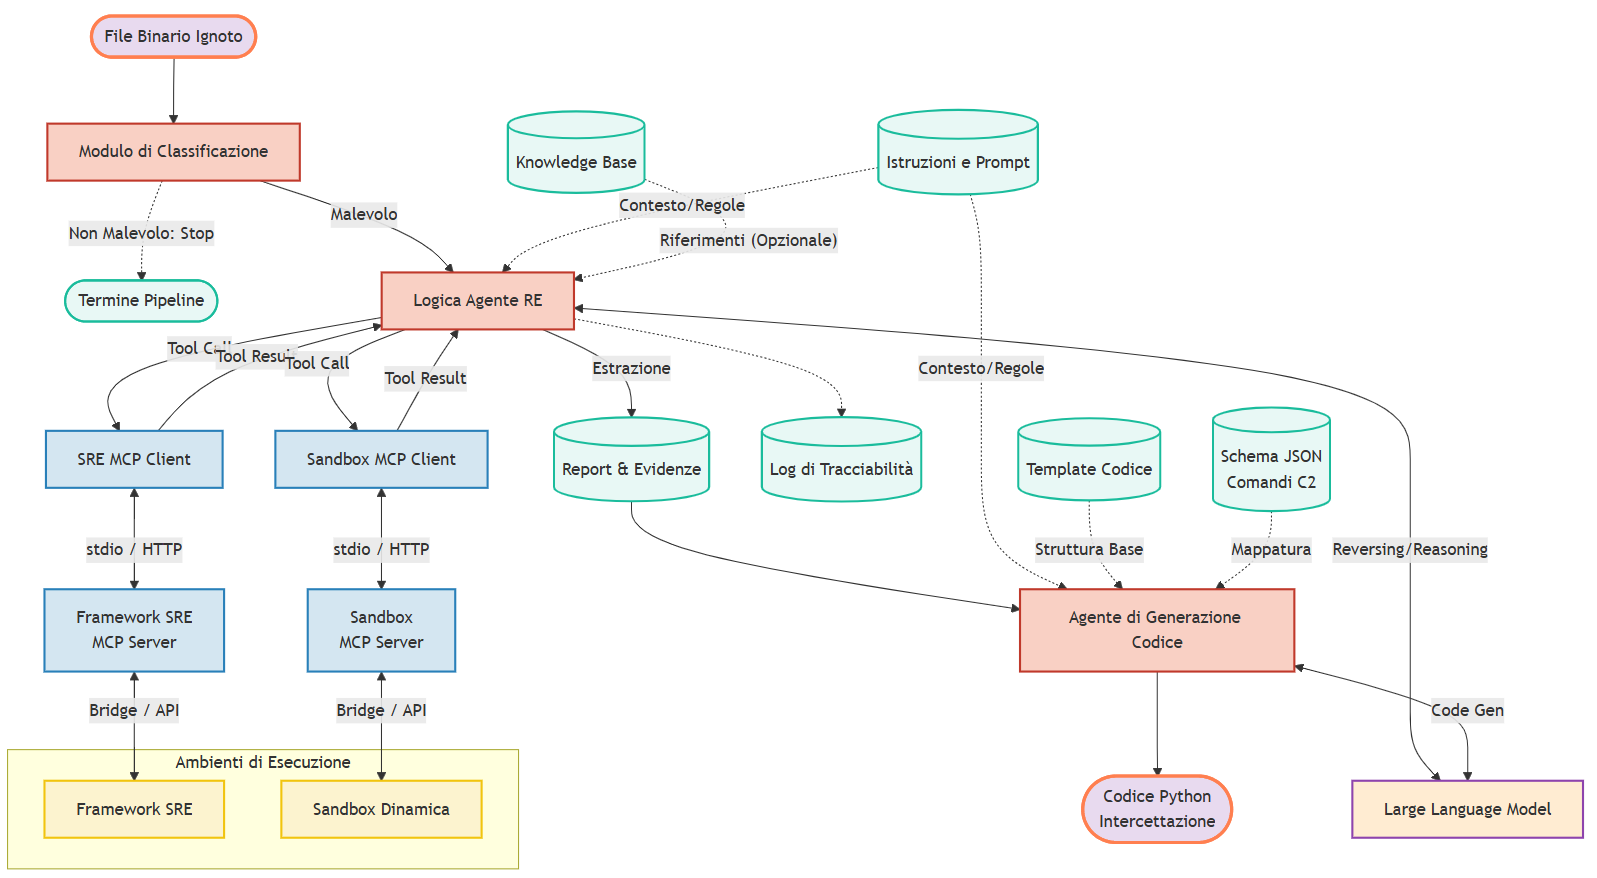
\includegraphics[scale=.35]{img/componenti.png}
    \caption{Diagramma UML dei componenti dell'architettura proposta}
    \label{fig:diagramma_componenti}
\end{figure}

\section{Componenti del sistema} % 4.2

In questa sezione vengono descritti nel dettaglio i singoli componenti che costituiscono l'architettura proposta. Per ciascuno di essi vengono individuati i principali requisiti, le responsabilità e le funzionalità messe a disposizione degli altri componenti del sistema. La descrizione segue l'organizzazione mostrata nel diagramma di \Cref{fig:diagramma_componenti}, in ordine di appartenenza alle diverse aree funzionali individuate.

\subsection{Artefatti} % 4.2.1

Il \binary{} e il \capture{} rappresentano rispettivamente l'input e l'output principale del sistema, mentre la \interface{} e lo \schema{} sono gli artefatti che formalizzano l'interfaccia e lo schema dei messaggi che il \capture{} deve rispettare. Tali elementi sono già stati introdotti e descritti diffusamente nel \Cref{chap:problema}, per cui nella fase di progettazione non è necessario aggiungere ulteriori dettagli.

I \file{} sono i file prodotti dal \sreagent{} durante le attività svolte nel \sandbox{}. Dal momento che sono generati da un \llm{} che interagisce con un malware, devono essere considerati \emph{untrusted} e, pertanto, non possono essere eseguiti automaticamente nel resto della pipeline. L'unica operazione consentita è la lettura in forma testuale dei file con estensioni considerate attendibili, mentre qualsiasi altra operazione su di essi può essere eseguita esclusivamente dall'utente.

I \logs{} permettono di tracciare in dettaglio le azioni svolte dal \llm{} all'interno del \sreagent{}, consentendo all'utente di effettuare una revisione delle operazioni eseguite durante l'analisi e supportando le attività di debugging. Possono essere costituiti da più tipologie di file, che riportano informazioni differenti e presentano livelli di strutturazione variabili.

% Nei casi previsti i \logs{} possono permettere di riprendere o continuare manualmente l'esecuzione a partire da uno stato precedente. Possono includere anche informazioni relative all'uso delle risorse computazionali e ai tempi di esecuzione.

I \templates{} rappresentano l'insieme dei template di codice che il \codeagent{} può utilizzare come riferimento per la creazione del \capture{}, secondo un approccio di few-shot prompting. Tra questi deve essere presente almeno un file principale contenente una classe che implementi la \interface{}, eventualmente affiancato da ulteriori file per modularizzare il codice e separare le responsabilità. Analogamente alla \kb{}, i \templates{} potrebbero inoltre essere declinati in versioni specifiche per ciascuna famiglia di botnet. L'introduzione dei \templates{} mira a standardizzare e strutturare, almeno in parte, l'output del sistema, limitando la variabilità del codice prodotto dal \llm{} anche a fronte di campioni simili, pur mantenendo una certa libertà implementativa. Inoltre, essi contribuiscono a ridurre il che rischio che il codice generato contenga funzionalità malevole, fornendo al \llm{} un esempio privo di tali funzionalità.

% ad esempio attraverso moduli specifici dedicati alla classificazione e al parsing dei messaggi

Il \prompt{} è pensato per raccogliere le istruzioni, system prompt e user prompt, che vengono fornite agli agenti AI di \sreagent{} e \codeagent{}. La funzione dei \emph{system prompt} \cite{dhamani2026genai} è quella di definire il ruolo dell'agente, il comportamento da assumere, il tono da utilizzare, i vincoli e le capacità previste per l'applicazione specifica. Gli \emph{user prompt} \cite{dhamani2026genai} descrivono nello specifico le attività che l'utente richiede al \llm{} di eseguire nel ruolo definito, insieme all'indicazione dell'output atteso e eventuali informazioni aggiuntive. A differenza dei prompt, che tendono a rimanere relativamente stabili nel tempo, come già anticipato la \kb{} è invece pensata per avere una natura maggiormente dinamica, potendo essere aggiornata o modificata in funzione delle esigenze del reverse engineer o dell'evoluzione delle conoscenze disponibili.
    
% Proprio per questa caratteristica, un'implementazione efficace potrebbe prevedere la raccolta di informazioni specifiche per le diverse famiglie di malware, che il \sreagent{} può utilizzare in funzione del singolo campione analizzato, evitando di incorporare direttamente nei prompt informazioni che possono variare da un campione all'altro. Il \sreagent{} deve comunque essere in grado di svolgere l'attività di analisi anche senza le informazioni della \kb{}.

I \report{} rappresentano l'artefatto chiave dell'intera pipeline dal momento che si collocano tra \sreagent{} e \codeagent{}. I report devono quindi sintetizzare con un elevato livello di dettaglio l'attività di SRE svolta dal \sreagent{} e, allo stesso tempo, fungere da \emph{single source of truth} (SSOT) per la successiva produzione del \capture{} da parte del \codeagent{}. In più i \report{} devono anche fornire una documentazione analizzabile e verificabile dall'utente, permettendogli di validare autonomamente quanto rilevato e correggere eventuali errori nel \capture{}. A questo scopo, è importante che ciascun documento sia organizzato in modo chiaro, eventualmente adottando un formato strutturato, per facilitarne la lettura da parte dell'utente e la comprensione da parte del \textsc{LLM}. Il contenuto deve inoltre riportare in dettaglio i risultati dell'analisi, attraverso una sequenza chiara di evidenze e riferimenti a supporto delle conclusioni raggiunte.

% Semistrutturato: ad esempio Markdown. Il contenuto deve inoltre utilizzare un linguaggio appropriato. Conclusioni raggiunte: ad esempio indirizzi di memoria e nomi utilizzati.

\subsection{Componenti decisionali} % 4.2.2

Il \llm{} costituisce la base per l'implementazione delle funzionalità previste dal \sreagent{} e dal \codeagent{}, agendo come motore cognitivo e fornendo le capacità necessarie alla comprensione, al ragionamento, alla pianificazione e, ove previsto, all'utilizzo dei tool. Dal punto di vista tecnico, il LLM utilizzato deve garantire prestazioni adeguate alle attività previste, con buone capacità di reasoning, il supporto nativo a tool call strutturate e una finestra di contesto sufficientemente ampia.

% (dimensioni sufficienti per il LLM e le tool call possono essere eventualmente emesse in parallelo)

Il \classifier{} agisce come \emph{gatekeeper} della pipeline di analisi e ha il compito di esaminare preliminarmente il \binary{} ricevuto, decidendo se instradarlo verso il \sreagent{} oppure interrompere prematuramente il flusso di analisi, per evitare l'impiego di risorse nello studio di campioni che non lo richiedono o che non risultano interessanti. Inoltre, pur non essendo necessario per il funzionamento di base, questo modulo può essere esteso per estrarre ulteriori informazioni preliminari che possono essere utilizzate per fornire al \sreagent{} un contesto più specifico, sfruttando la \kb{}.

% Identificazione di informazioni preliminari, come l'identificazione della famiglia di botnet a cui appartiene il campione.

Il \sreagent{} si occupa di orchestrare l'attività di SRE sul \binary{}, in accordo con le istruzioni recuperate dal \prompt{} e, quando disponibili, con le conoscenze aggiuntive contenute nella \kb{}. A tal fine pianifica la strategia di analisi, la esegue attraverso i tool messi a disposizione dal \sreframework{} e dalla \sandbox{}, e infine riassume le informazioni raccolte all'interno dei \report{}. Il modulo è inoltre responsabile della gestione del collegamento tra l'agente e gli ambienti di esecuzione mediante il protocollo MCP, inoltrando le tool call generate dal \llm{} ai rispettivi MCP client e restituendo i risultati delle operazioni eseguite. Infine, il \sreagent{} deve implementare le funzionalità di logging richieste e deve adattare il proprio comportamento in funzione del fatto che il campione analizzato sia stripped o not-stripped.

Il \codeagent{} guida e coordina le attività di generazione del \capture{}, sulla base delle istruzioni definite nei relativi prompt. Come input riceve i \report{}, lo \schema{} e i \templates{}, che includono anche la \interface{}. A partire dall'insieme di questi elementi, il \codeagent{} deve estrarre e combinare le informazioni necessarie per costruire il \capture{} conforme ai requisiti strutturali e di sicurezza previsti.

% L'agente è pertanto responsabile di produrre un modulo funzionante e conforme ai formati e alle strutture richieste, in particolare rispettando l'interfaccia prevista e senza introdurre alcuna capacità offensiva.

\subsection{Integrazione MCP} % 4.2.3

Il \textsc{SRE MCP Server} e il \textsc{Sandbox MCP Server} sono i server MCP dedicati ai due ambienti di esecuzione del sistema ed espongono i tools che potranno essere utilizzati dal \sreagent{}.  Ogni tool \cite{anthropic2024mcp} deve avere un \emph{name} univoco che permette di identificare chiaramente il suo scopo, un \emph{title} opzionale, una \emph{description} delle modalità di utilizzo e infine un \emph{inputSchema}, un JSON Schema che specifica, per ciascun parametro di input, il tipo, la relativa descrizione e se è obbligatorio (\emph{required}) o opzionale. I server devono inoltre predisporre il meccanismo di trasporto attraverso cui accettare le connessioni dei client, utilizzando il protocollo \texttt{stdio} nel caso di client locali oppure \texttt{Streamable HTTP} nel caso di client remoti. A fronte delle richieste di esecuzione dei tool ricevute dai client, il server deve effettuare il \emph{dispatch} verso la relativa implementazione e, dopo l'esecuzione, deve restituire il risultato in un formato prestabilito.

% L'implementazione può essere realizzata direttamente oppure indirettamente, delegando l'operazione effettiva a un altro componente.
% https://modelcontextprotocol.io/docs/2026-07-28/learn/architecture#understanding-the-tool-discovery-response

Il \textsc{SRE MCP Client} e il \textsc{Sandbox MCP Client} sono i client MCP associati ai rispettivi server MCP. Ciascun client, utilizzando gli \emph{endpoint} \texttt{tools/list} e \texttt{tools/call} del server, deve esporre le funzionalità che permettano a un agente AI di scoprire i tool disponibili e di invocare un tool, specificandone il nome e gli eventuali argomenti. % \texttt{name}, una stringa, e gli eventuali \texttt{arguments}, rappresentati da un oggetto JSON.

% Dal momento che l'utilizzatore di tali funzionalità sarà il \llm{} all'interno del \sreagent{}, può inoltre essere utile prevedere due funzionalità di parsing personalizzate. La prima riguarda la conversione della descrizione dei tool disponibili dal formato di schema standard MCP al formato accettato dal \llm{}. La seconda può riguardare la formattazione specifica di alcune risposte ricevute dai tool.

% https://modelcontextprotocol.io/specification/2026-07-28/server/tools#listing-tools
% https://modelcontextprotocol.io/specification/2026-07-28/server/tools#calling-tools

% Tutto in conformità al protocollo MCP.

\subsection{Ambienti di esecuzione} % 4.2.4

Il \sreframework{} deve disporre di funzionalità proprie dei sistemi di SRE, tra cui il disassemblaggio, la decompilazione e, ove necessario, il debugging, così da fornire al \sreagent{} le capacità necessarie per svolgere le attività di analisi statica del codice e, eventualmente, di analisi dinamica avanzata. Tra gli strumenti per l'analisi statica da esporre rientrano, a titolo esemplificativo, l'analisi e la gestione delle funzioni e delle relative \emph{cross-reference}, degli indirizzi e della memoria, del \emph{type system}, nonché la gestione e la rinomina dei simboli. 

Il \sandbox{} ha lo scopo di mettere a disposizione funzionalità dinamiche aggiuntive per l'analisi, potenzialmente diverse da quelle offerte dalle classiche attività di esecuzione o debugging, così da poter essere affiancato e combinato al \sreframework. All'interno dell'architettura proposta, il \sandbox{} rappresenta un ambiente generale nel quale, durante il processo di SRE, è possibile costruire ed eseguire strumenti personalizzati per trasformare, analizzare e interpretare le informazioni estratte durante l'analisi, oppure per automatizzare determinate attività. Uno degli aspetti più critici dell'implementazione di questo componente consiste nell'assicurare la sicurezza dell'ambiente. La sandbox deve garantire l'isolamento dall'host, operare con privilegi minimi e prevedere limiti alle risorse computazionali disponibili. L'accesso alla rete dovrebbe essere negato per impostazione predefinita e consentito esclusivamente qualora l'implementazione garantisca adeguate condizioni di sicurezza.

% La sandbox deve inoltre permettere di operare a livello di file, effettuando operazioni di lettura e scrittura secondo le necessità. Deve essere anche garantito l'isolamento da eventuali altre esecuzioni.

Per entrambi gli ambienti di esecuzione, ai fini dell'integrazione con il \llm{} all'interno del \sreagent{}, è fondamentale che le funzionalità offerte siano esposte attraverso un'interfaccia che ne consenta l'accesso tramite il protocollo MCP. % , ad esempio mediante plugin o API,

\section{Flusso di esecuzione} % 4.3

Dopo aver descritto la struttura complessiva dell'architettura di \system{} e le responsabilità dei singoli componenti, questa sezione illustra il flusso di esecuzione completo, ripercorrendo le attività che si susseguono a partire dal \binary{} di input e mostrando il percorso seguito attraverso i diversi componenti del sistema, fino ad arrivare alla produzione del \capture{}.

A questo scopo viene utilizzato un diagramma UML delle attività \cite{omg2017uml}, un diagramma comportamentale che permette di rappresentare lo svolgimento di un processo attraverso il flusso delle attività, le decisioni, i percorsi alternativi, le attività eseguite in parallelo e, ove necessario, il flusso degli oggetti. % Capitolo 15

Il diagramma delle attività realizzato è riportato in \Cref{fig:diagramma_attivita}. A differenza del diagramma dei componenti presentato nella sezione precedente, questo diagramma ha una finalità esclusivamente descrittiva: rappresenta infatti un flusso semplificato utilizzato solamente per illustrare il comportamento del sistema e non costituisce una specifica vincolante per l'implementazione.

\begin{figure}[t]
    \centering
    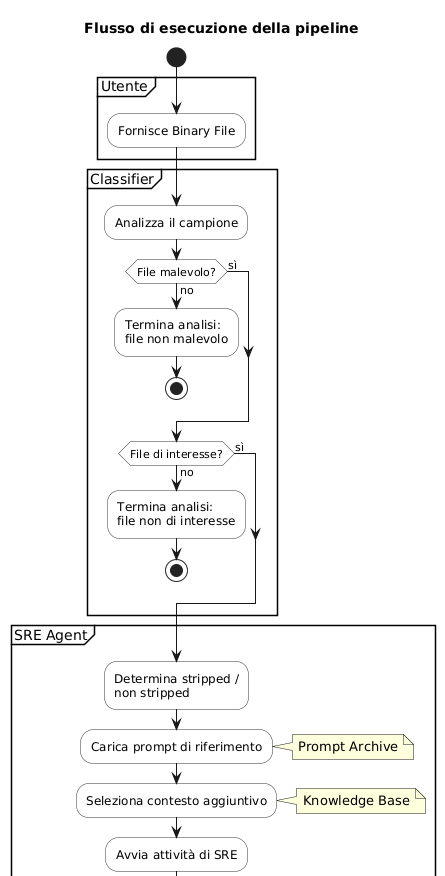
\includegraphics[scale=.60]{img/attivita_1.png}
    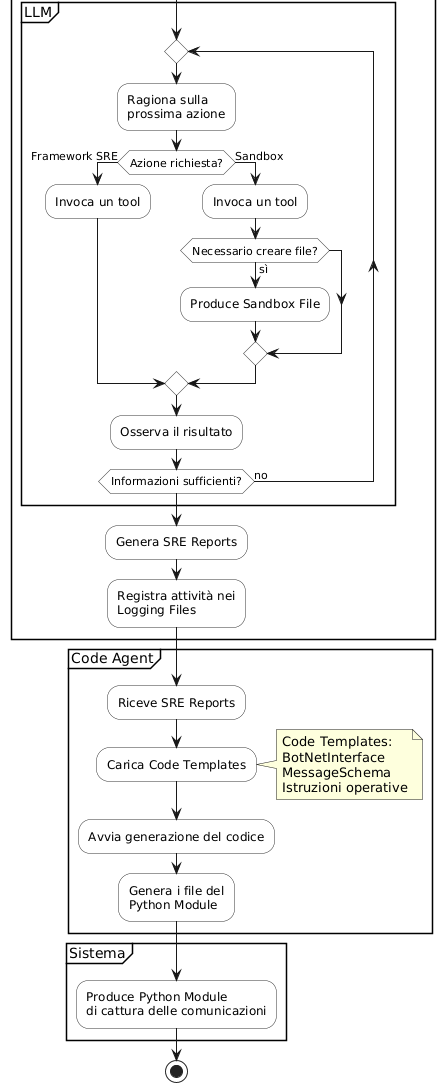
\includegraphics[scale=.45]{img/attivita_2.png}
    \caption{Diagramma UML delle attività della pipeline di analisi}
    \label{fig:diagramma_attivita}
\end{figure}

Il flusso di esecuzione ha inizio quando l'utente fornisce in ingresso al sistema il \binary{}. Quindi, il \classifier{} ne esegue un'analisi preliminare, finalizzata almeno a determinare se il campione sia malevolo oppure no. Quando è possibile stabilire con certezza che il campione non è malevolo oppure che, pur essendo malevolo, non è di interesse per il sistema, allora la pipeline di analisi viene interrotta. Negli altri casi il campione viene trasferito dal \classifier{} al \sreagent{}.

Come prima cosa, il \sreagent{}, basandosi sulla presenza dei simboli, determina se il campione è stripped o not-stripped. Nel primo caso, l'agente potrebbe subito svolgere qualche azione apposita oppure adatterà di conseguenza il proprio comportamento durante le attività di SRE. A questo punto l'agente carica le istruzioni dal \prompt{} e, quando possibile, utilizza le informazioni aggiuntive rese disponibili dal \classifier{} per selezionare dalla \kb{} il contesto supplementare pertinente al campione.

La fase centrale è dunque costituita dall'attività di SRE svolta dal \sreagent{} attraverso il \llm{}, secondo un ciclo iterativo di ragionamento, azione e osservazione. Per fare ciò, il modello utilizza i tool messi a disposizione dagli ambienti \sreframework{} e \sandbox{}, interagendoci attraverso il protocollo MCP. Nel caso del \sandbox{}, il \llm{} potrà anche produrre e salvare dei \file{}. Quando l'agente dispone di informazioni sufficienti, conclude l'analisi, producendo i \report{}, mentre le attività svolte vengono registrate nei \logs{}.

Infine, i \report{} vengono passati al \codeagent{}, che carica i \templates{}, lo schema dei messaggi e le istruzioni operative dal \prompt{}. Il \llm{} dell'agente utilizza questa serie di informazioni per generare gli elementi necessari a costruire il \capture{} di cattura delle comunicazioni, che corrisponde all'output finale del sistema.

\section{Tool calling} % 4.4

Considerata la rilevanza del meccanismo di \textit{tool calling} nell'architettura proposta e la frequenza con cui viene coinvolto durante l'attività di SRE, risulta utile fornire una rappresentazione più dettagliata delle interazioni che avvengono tra il \sreagent{} e gli ambienti di esecuzione mediante il protocollo MCP. I diagrammi dei componenti e di attività precedenti non rappresentano in efficace la natura di tali interazioni, per cui si utilizza un diagramma UML di sequenza \cite{omg2017uml}, un diagramma comportamentale che rappresenta come diversi componenti interagiscono tra loro nel corso del tempo, descrivendo lo scambio di messaggi ed evidenziando l'ordine temporale degli eventi. % Capitolo 17, 17.8 (relativo a una determinata interazione)

Il diagramma di sequenza realizzato è riportato in \Cref{fig:sequenza}. Esso rappresenta una sequenza esemplificativa, corrispondente solamente a un sottoinsieme delle interazioni che si verificano durante le attività di analisi da parte del \textsc{SRE Agent}.

\begin{figure}[t]
    \centering
    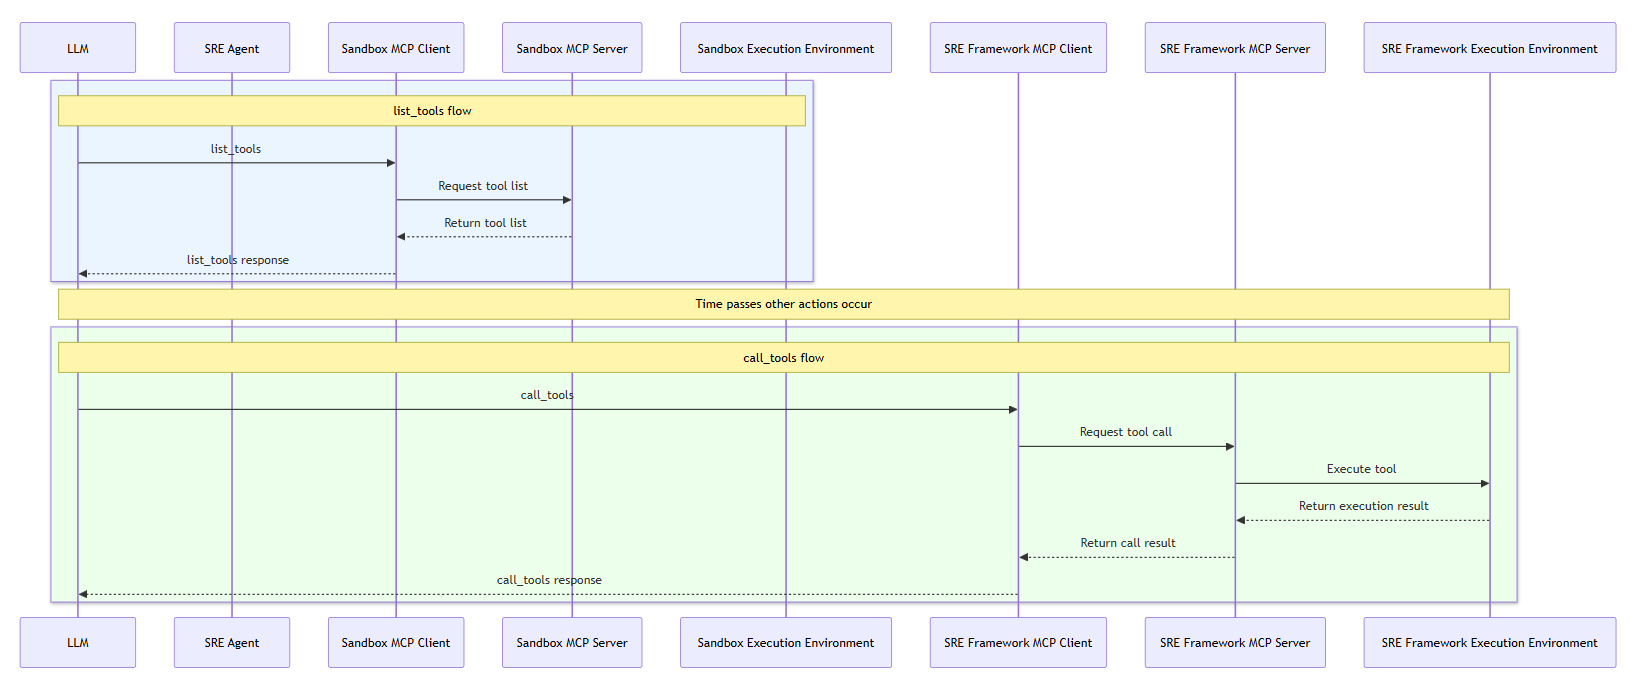
\includegraphics[scale=.35]{img/sequenza.png}
    \caption{Diagramma UML di sequenza delle operazioni di tool calling}
    \label{fig:sequenza}
\end{figure}

Il diagramma mostra nella prima parte della sequenza alcune delle operazioni preliminari relative alla creazione e alla configurazione degli oggetti coinvolti nelle interazioni successive, tra cui l'istanziazione dei client MCP e del \llm{} da parte del \sreagent{}.

La seconda parte della sequenza riguarda la scoperta dei tool disponibili per l'ambiente \sandbox{} da parte dell'agente. Il \sreagent{} richiede al \textsc{Sandbox MCP Client} la lista dei tool tramite la funzione $list\_tools()$ e il client invoca quindi l'endpoint \texttt{tools/list} del \textsc{Sandbox MCP Server}, che restituisce la lista dei tool secondo il formato previsto dal protocollo MCP. Il client può eventualmente convertire il formato della risposta in quello richiesto dal \llm{}, restituendo quindi la lista al \sreagent{}. Quest'ultimo può utilizzare la lista ottenuta come parametro per le richieste inviate al \llm{}, eventualmente limitandola anche a un sottoinsieme dei tool disponibili.

La terza parte riguarda invece l'effettiva chiamata di un generico tool del \sreframework{}. Il \sreagent{}, dopo aver invocato il \llm{}, riceve una risposta strutturata contenente una o più tool call, le estrae e determina a quale ambiente di esecuzione appartengano. Nel caso considerato, la chiamata riguarda il \sreframework{}, per cui l'agente richiede al \textsc{SRE MCP Client} l'esecuzione del tool tramite la funzione $call\_tool(name, arguments)$. Il client invoca quindi l'endpoint \texttt{tools/call} del \textsc{SRE MCP Server}, specificando il $name$ del tool e gli eventuali $arguments$ come oggetto JSON. Ricevuta la richiesta il \textsc{SRE MCP Server} provvede a gestirla, avviando l'esecuzione dell'operazione corrispondente sul \sreframework{}. Quando quest'ultima termina, il \sreframework{} restituisce il relativo risultato al server, che può eventualmente formattarlo prima di restituirlo al \textsc{SRE MCP Client}. Il client lo ritorna a sua volta al \sreagent{}, che può inserire il risultato del tool nel contesto del \llm{}, così da proseguire con l'attività di analisi.

% Tool call delimitate, ad esempio, dai tag $<tool_call>$ e $</tool_call>$.